\documentclass[border=10pt]{standalone}
\usepackage{tikz}
\usetikzlibrary{shapes.geometric, arrows.meta, positioning, fit, backgrounds}

\tikzset{
    box/.style={
        rectangle, draw=black, thick,
        minimum width=3.4cm, minimum height=0.85cm,
        align=center, font=\small
    },
    arrow/.style={->, >=Stealth, thick},
    grouplabel/.style={font=\small\itshape}
}

\begin{document}
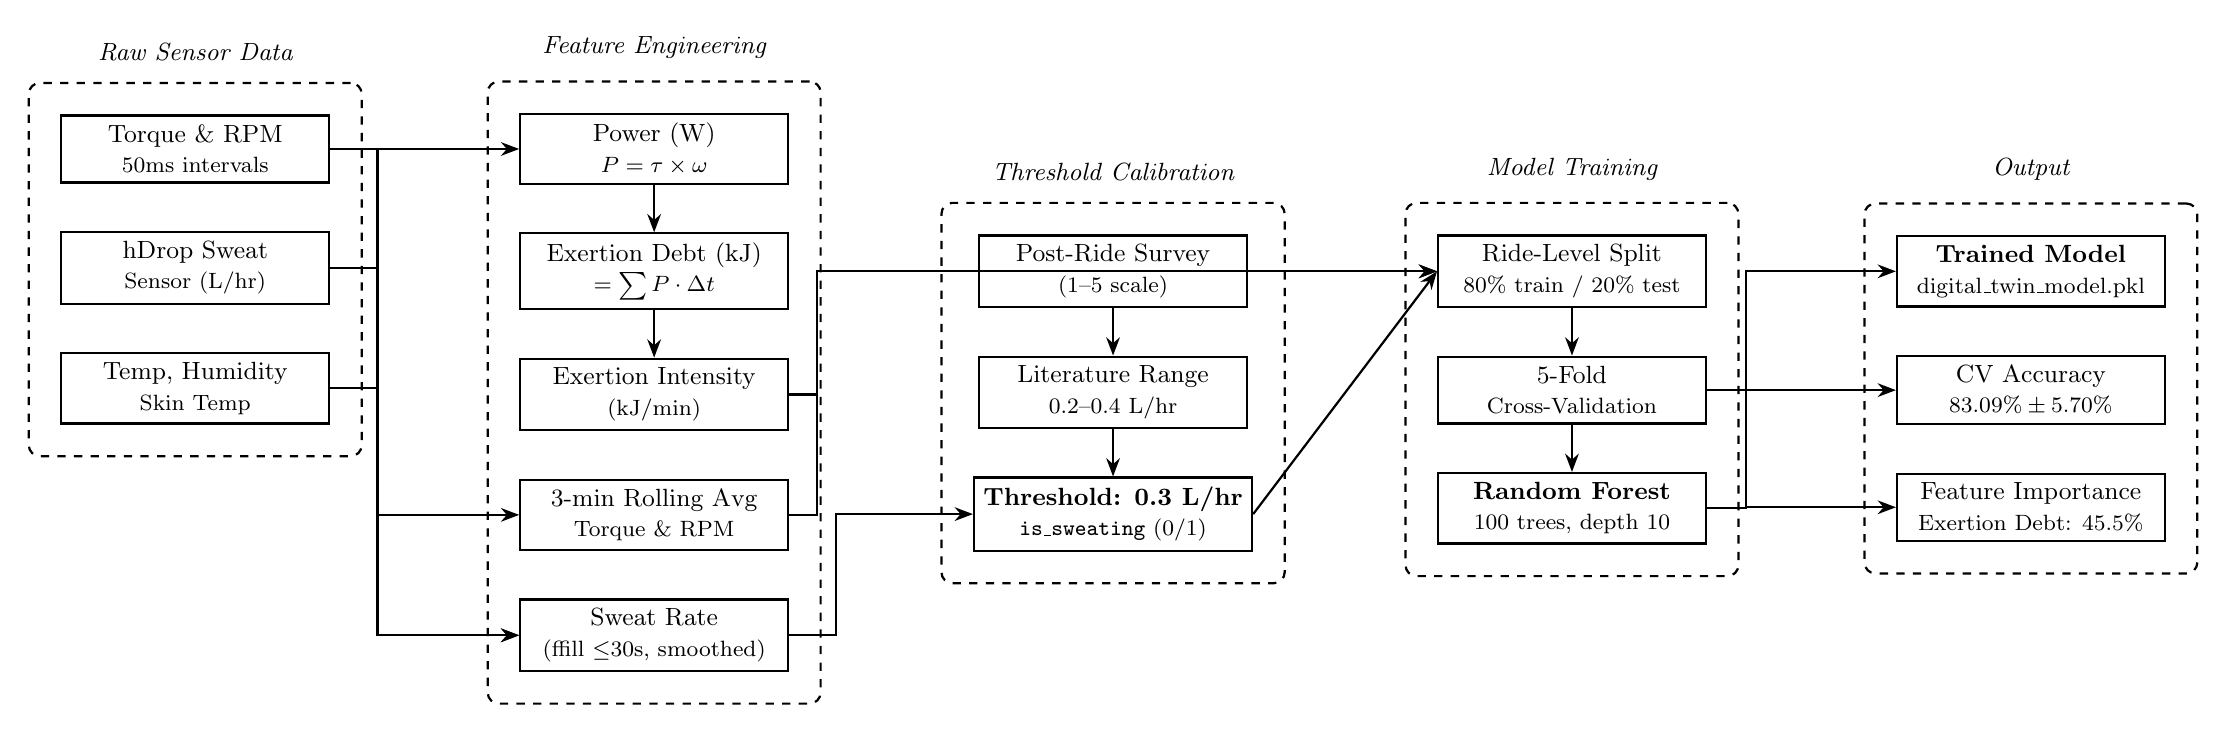
\begin{tikzpicture}[node distance=0.7cm and 2.2cm]

% ── Col 1: Raw Data ──────────────────────────────────────────────────────────
\node[box] (torque) {Torque \& RPM\\{\footnotesize 50ms intervals}};
\node[box, below=0.6cm of torque] (sweat) {hDrop Sweat\\{\footnotesize Sensor (L/hr)}};
\node[box, below=0.6cm of sweat] (env) {Temp, Humidity\\{\footnotesize Skin Temp}};

\begin{scope}[on background layer]
\node[draw=black, dashed, thick, rounded corners=4pt,
      fit=(torque)(env), inner sep=0.4cm] (g1) {};
\end{scope}
\node[grouplabel, above=0.15cm of g1] {Raw Sensor Data};

% ── Col 2: Feature Engineering ───────────────────────────────────────────────
\node[box, right=2.4cm of torque] (power)
    {Power (W)\\{\footnotesize $P = \tau \times \omega$}};
\node[box, below=0.6cm of power] (debt)
    {Exertion Debt (kJ)\\{\footnotesize $= \sum P \cdot \Delta t$}};
\node[box, below=0.6cm of debt] (intensity)
    {Exertion Intensity\\{\footnotesize (kJ/min)}};
\node[box, below=0.6cm of intensity] (rolling)
    {3-min Rolling Avg\\{\footnotesize Torque \& RPM}};
\node[box, below=0.6cm of rolling] (ffill)
    {Sweat Rate\\{\footnotesize (ffill $\leq$30s, smoothed)}};

\begin{scope}[on background layer]
\node[draw=black, dashed, thick, rounded corners=4pt,
      fit=(power)(ffill), inner sep=0.4cm] (g2) {};
\end{scope}
\node[grouplabel, above=0.15cm of g2] {Feature Engineering};

% ── Col 3: Threshold Calibration ─────────────────────────────────────────────
\node[box, right=2.4cm of debt] (survey)
    {Post-Ride Survey\\{\footnotesize (1--5 scale)}};
\node[box, below=0.6cm of survey] (lit)
    {Literature Range\\{\footnotesize 0.2--0.4 L/hr}};
\node[box, below=0.6cm of lit] (thresh)
    {\textbf{Threshold: 0.3 L/hr}\\{\footnotesize \texttt{is\_sweating} (0/1)}};

\begin{scope}[on background layer]
\node[draw=black, dashed, thick, rounded corners=4pt,
      fit=(survey)(thresh), inner sep=0.4cm] (g3) {};
\end{scope}
\node[grouplabel, above=0.15cm of g3] {Threshold Calibration};

% ── Col 4: Model Training ─────────────────────────────────────────────────────
\node[box, right=2.4cm of survey] (split)
    {Ride-Level Split\\{\footnotesize 80\% train / 20\% test}};
\node[box, below=0.6cm of split] (cv)
    {5-Fold\\{\footnotesize Cross-Validation}};
\node[box, below=0.6cm of cv] (rf)
    {\textbf{Random Forest}\\{\footnotesize 100 trees, depth 10}};

\begin{scope}[on background layer]
\node[draw=black, dashed, thick, rounded corners=4pt,
      fit=(split)(rf), inner sep=0.4cm] (g4) {};
\end{scope}
\node[grouplabel, above=0.15cm of g4] {Model Training};

% ── Col 5: Output ─────────────────────────────────────────────────────────────
\node[box, right=2.4cm of split] (model)
    {\textbf{Trained Model}\\{\footnotesize digital\_twin\_model.pkl}};
\node[box, below=0.6cm of model] (acc)
    {CV Accuracy\\{\footnotesize $83.09\% \pm 5.70\%$}};
\node[box, below=0.6cm of acc] (fimp)
    {Feature Importance\\{\footnotesize Exertion Debt: 45.5\%}};

\begin{scope}[on background layer]
\node[draw=black, dashed, thick, rounded corners=4pt,
      fit=(model)(fimp), inner sep=0.4cm] (g5) {};
\end{scope}
\node[grouplabel, above=0.15cm of g5] {Output};

% ── Arrows: Col 1 → Col 2 ────────────────────────────────────────────────────
\draw[arrow] (torque.east) -- (power.west);
\draw[arrow] (torque.east) -- ++(0.6,0) |- (rolling.west);
\draw[arrow] (sweat.east)  -- ++(0.6,0) |- (ffill.west);
\draw[arrow] (env.east)    -- ++(0.6,0) |- (ffill.west);

% ── Arrows: within Col 2 ─────────────────────────────────────────────────────
\draw[arrow] (power.south)     -- (debt.north);
\draw[arrow] (debt.south)      -- (intensity.north);

% ── Arrows: Col 2 → Col 3 ────────────────────────────────────────────────────
\draw[arrow] (ffill.east) -- ++(0.6,0) |- (thresh.west);

% ── Arrows: within Col 3 ─────────────────────────────────────────────────────
\draw[arrow] (survey.south) -- (lit.north);
\draw[arrow] (lit.south)    -- (thresh.north);

% ── Arrows: Col 2 → Col 4 (features feed training) ───────────────────────────
\draw[arrow] (intensity.east) -- ++(0.35,0) |- (split.west);
\draw[arrow] (rolling.east)   -- ++(0.35,0) |- (split.west);

% ── Arrow: Col 3 → Col 4 (threshold provides labels) ─────────────────────────
\draw[arrow] (thresh.east) -- (split.west);

% ── Arrows: within Col 4 ─────────────────────────────────────────────────────
\draw[arrow] (split.south) -- (cv.north);
\draw[arrow] (cv.south)    -- (rf.north);

% ── Arrows: Col 4 → Col 5 ────────────────────────────────────────────────────
\draw[arrow] (rf.east)  -- ++(0.5,0) |- (model.west);
\draw[arrow] (cv.east)  -- ++(0.5,0) |- (acc.west);
\draw[arrow] (rf.east)  -- ++(0.5,0) |- (fimp.west);

\end{tikzpicture}
\end{document}
